We model our ER diagram (\cref{fig:er-diagram}) after Pomona College's current
room draw system with a few modifications. A \emph{Student} is required to be
a part of at least one \emph{DrawGroup}, which consists of one or more
students. We gave draw groups a specific draw number attribute to distinguish
between normal draw and suite draw, the latter averaging individual student draw
numbers.

Furthermore, each draw group must have a \emph{Representative} who
will select a \emph{Collection} of one or more rooms for the group, depending
on the size of the group. All students are representatives of themselves in a
group containing only themselves.

Similar to the student/draw group coupling, a
\emph{Room} is required to be a part of exactly one collection. These
collections represent individual rooms and multiple associated rooms such as
two-room doubles and friendship suites. A representative may \emph{Request} a
collection and rank the request for automated room draw; this ranking makes up
the group's preference's list. If any of the collections specified on the
representative student's preferences list are available at the representative's
draw time, the highest ranked available collection will be drawn for the group.
These draw times correspond to a group's absolute rank attribute which is
determined by whether or not the group is a friendship suite and by the group's
draw number.

Just as a note, not every draw group participate in the \emph{Request
} relation as groups containing student abroad will not have a preferences list
for the semester they are abroad. Along the same vein, not all rooms on Pomona's
campus are occupied at any given time so not all collections will participate in the \emph{Request} relationship. For the same reasons, the \emph{Occupy} relationship does not require total participation by either students or rooms.

\begin{figure}[H] \centering
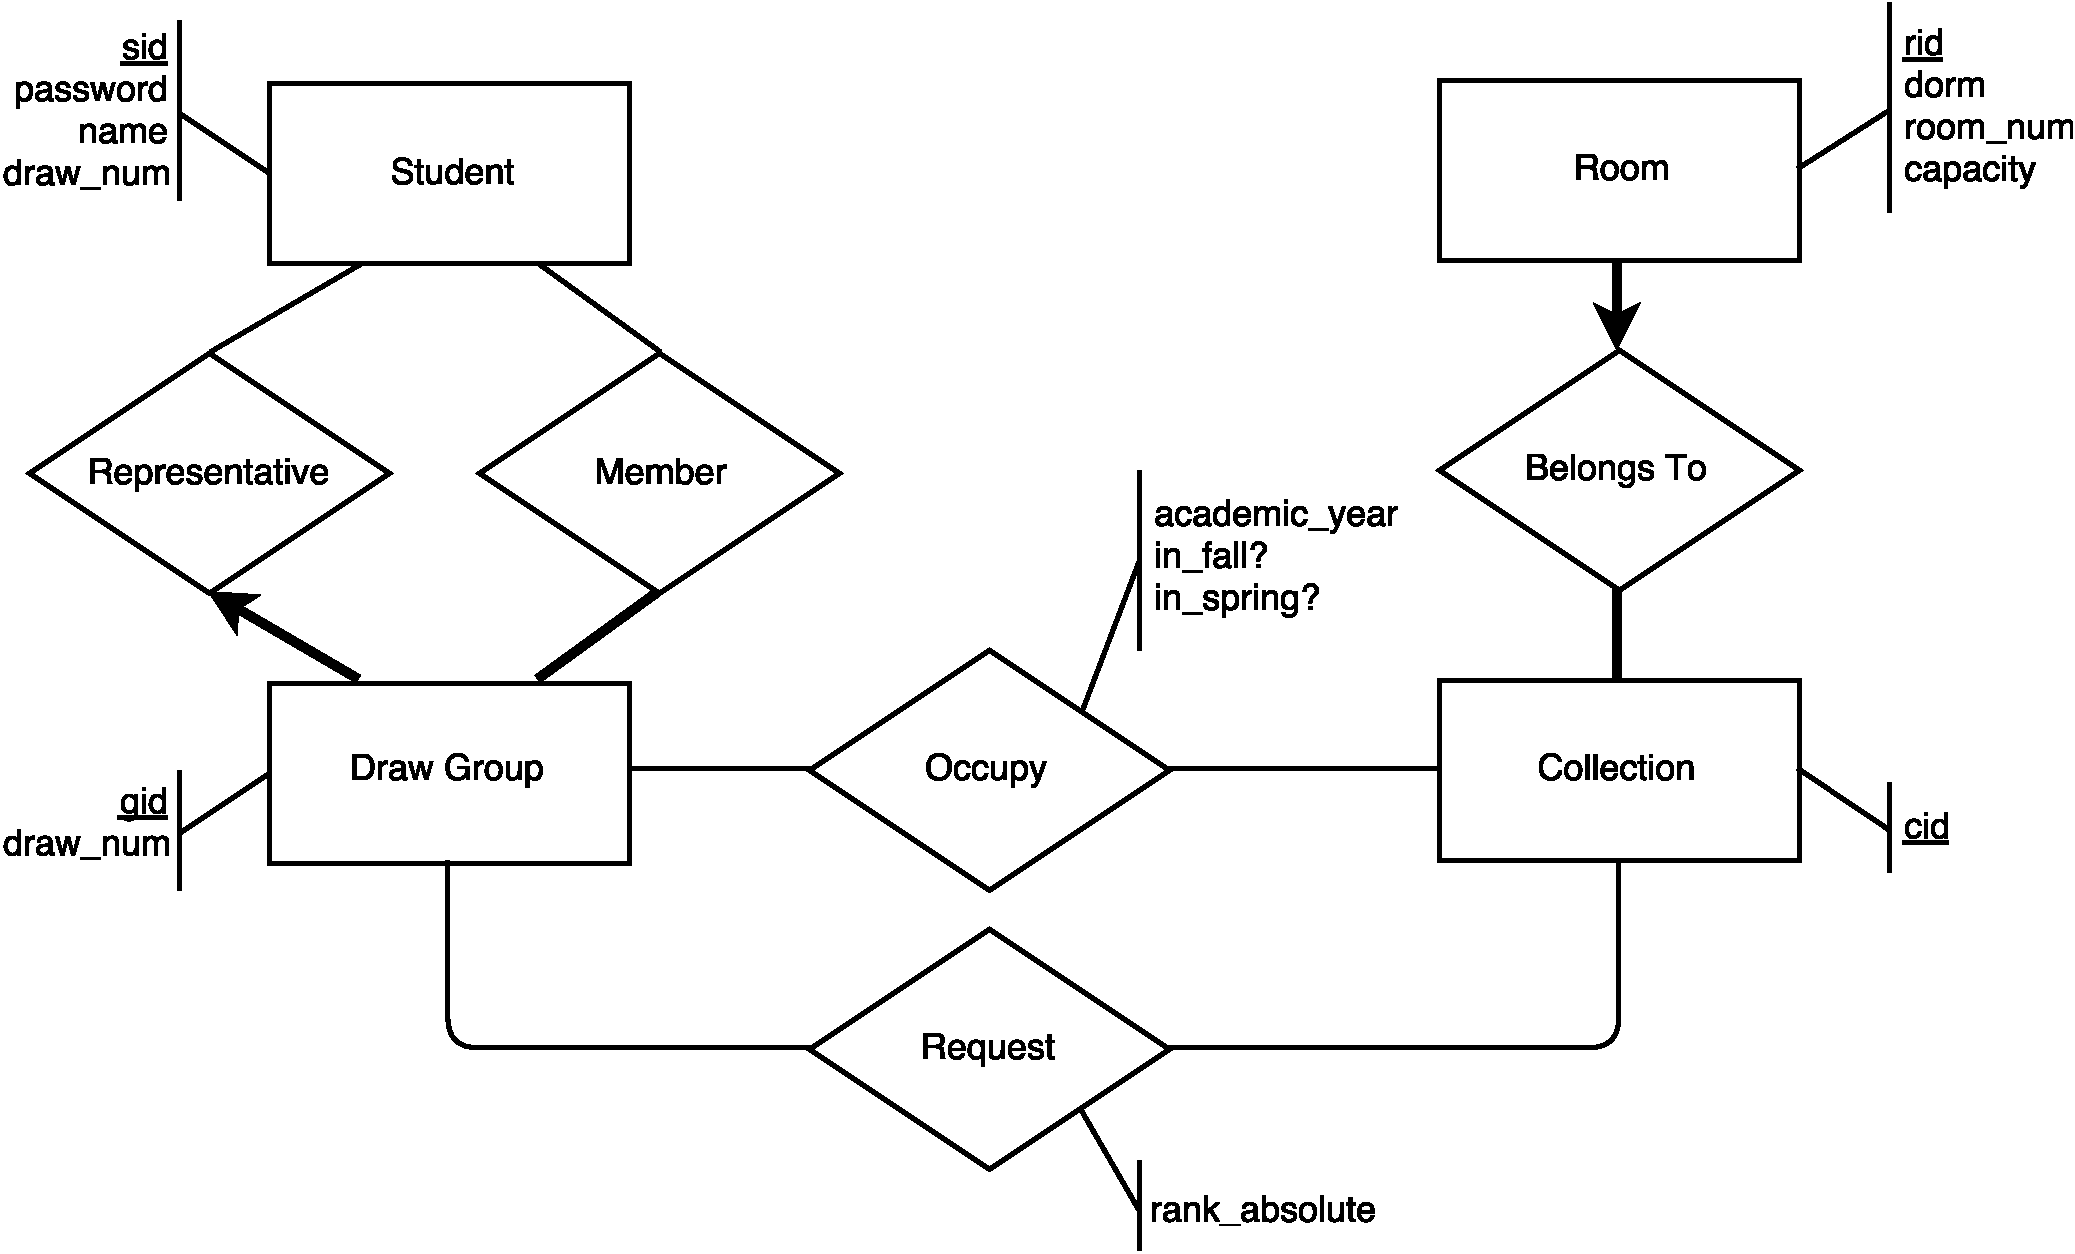
\includegraphics[width=\textwidth]{er_crop.pdf}
\caption{Our ER Diagram}
\label{fig:er-diagram}
\end{figure}
